\section{辛普森悖论（Simpson's Paradox）}

\begin{frame}{Simpson's Paradox: COVID-27}
\href{https://www.youtube.com/playlist?list=PLoazKTcS0RzZ1SUgeOgc6SWt51gfT80N0}{Brady Neal}的slides中用COVID-27的例子说明了Simpson's Paradox。这个例子与\textcite{GLSJ202510012}中"分块随机化实验"的思想在底层原理上完全一致。

\vspace{0.5em}

  \begin{table}
  \centering
  \renewcommand{\arraystretch}{1.3} % 增加行距，防止幻灯片中显得拥挤
  \setlength{\tabcolsep}{10pt}      % 调整列间距
  \begin{tabular}{lccc}
    \toprule
    % 第一列表头跨2行，后面三列的上方加一个跨3列的总表头
    \multirow{2}{*}{\textbf{Treatment}} & \multicolumn{3}{c}{\textbf{Condition}} \\
    \cmidrule(lr){2-4} % 在第2列到第4列下方画一条修饰用的短横线，(lr)表示左右两端稍微缩进
    & \textbf{Mild} & \textbf{Severe} & \textbf{Total} \\
    \midrule
    Treatment A & 210/1400 = 15\% & 30/100 = 30\% & 240/1500 = 16\% \\
    Treatment B & 5/50 = 10\%    & 100/500 = 20\% & 105/550 = 19.1\% \\
    \bottomrule
  \end{tabular}
\end{table}


  朴素比较（不分层）：A的死亡率16\%低于B的19.1\%，A看起来更好。但在每一层内部：轻症中B（10\%）优于A（15\%），重症中B（20\%）优于A（30\%）。这就是Simpson's Paradox——总体趋势与分层趋势方向相反。

\vspace{2em}
\end{frame}

% ============================================================
% Frame 1：问题引入 + Scenario 1（Confounder）
% ============================================================
\begin{frame}{Scenario 1：C 是 Confounder}

  \begin{columns}[c]
    \begin{column}{0.55\textwidth}
      \begin{itemize}
        \item 因果图：$C \to T$，$C \to Y$，$T \to Y$
        \item 病情 $C$ 是\textbf{混杂变量}，同时影响治疗选择和结果
        \item \textbf{应该控制} $C$
      \end{itemize}

      \medskip

      \begin{exampleblock}{直觉}
        新冠疫情中，轻症患者进方舱接受传统医学干预，重症患者进ICU接受现代医学干预。病情严重程度同时决定了治疗分配和死亡率，直接对比两种处理有失公允。
      \end{exampleblock}
    \end{column}

    \begin{column}{0.4\textwidth}
      \centering
      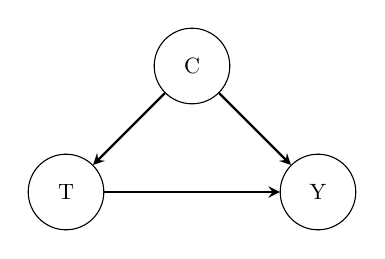
\begin{tikzpicture}[scale=0.8, every node/.style={scale=0.8}]
        \tikzstyle{circ} = [draw, circle, minimum size=1.2cm, align=center, inner sep=1pt]
        \node[circ] (T) at (0, 0) {T};
        \node[circ] (Y) at (4, 0) {Y};
        \node[circ] (C) at (2, 2) {C};
        \draw[->, >=stealth, thick] (C) -- (T);
        \draw[->, >=stealth, thick] (C) -- (Y);
        \draw[->, >=stealth, thick] (T) -- (Y);
      \end{tikzpicture}
    \end{column}
  \end{columns}

\end{frame}

% ============================================================
% Frame 2：Scenario 2（Mediator）
% ============================================================
\begin{frame}{Scenario 2：C 是 Mediator}

  \begin{columns}[c]
    \begin{column}{0.55\textwidth}
      \begin{itemize}
        \item 因果图：$T \to C \to Y$，$T \to Y$
        \item 治疗 $T$ 影响病情 $C$（如副作用导致病情加重），$C$ 是\textbf{中介变量}
        \item \textbf{不应该控制} $C$
      \end{itemize}

      \medskip

      \begin{exampleblock}{直觉}
        如果 Treatment B 需要患者等待很长时间，等待本身导致病情加重，那么"病情加重"是治疗的后果，不是预先存在的混杂。在回归中控制它会遮蔽治疗的真实总效应。
      \end{exampleblock}
    \end{column}

    \begin{column}{0.4\textwidth}
      \centering
      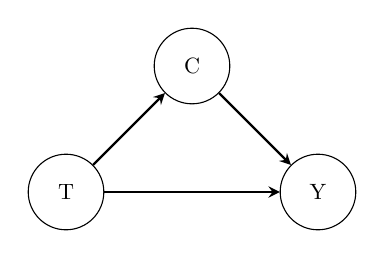
\begin{tikzpicture}[scale=0.8, every node/.style={scale=0.8}]
        \tikzstyle{circ} = [draw, circle, minimum size=1.2cm, align=center, inner sep=1pt]
        \node[circ] (T) at (0, 0) {T};
        \node[circ] (Y) at (4, 0) {Y};
        \node[circ] (C) at (2, 2) {C};
        \draw[->, >=stealth, thick] (T) -- (C);
        \draw[->, >=stealth, thick] (C) -- (Y);
        \draw[->, >=stealth, thick] (T) -- (Y);
      \end{tikzpicture}
    \end{column}
  \end{columns}

\end{frame}

% ============================================================
% Frame 3：对比表格 + 效应分解 + 核心启示
% ============================================================
\begin{frame}[allowframebreaks]{同样的数据，完全相反的结论}

  \begin{table}
  \centering
  \begin{tabular}{l|c|c}
    \hline
     & \textbf{Scenario 1 (Confounder)} & \textbf{Scenario 2 (Mediator)} \\
    \hline
    因果图 & $C \to T$，$C \to Y$，$T \to Y$ & $T \to C \to Y$，$T \to Y$ \\
    观测数据 & 完全相同 & 完全相同 \\
    应该控制C吗 & \checkmark{} 应该 & $\times$ 不应该 \\
    \texttt{reg Y T} 的系数 & +0.031（$\times$ 有偏） & +0.031（\checkmark{} 无偏） \\
    \texttt{reg Y T C} 的系数 & $-$0.082（\checkmark{} 无偏） & $-$0.082（$\times$ 有偏） \\
    正确的因果效应 & $-$0.065 & +0.031 \\
    应该选择 & \textbf{Treatment B} & \textbf{Treatment A} \\
    \hline
  \end{tabular}
  \caption{两个Scenario的结果对比}
  \end{table}

  \begin{block}{效应分解（Scenario 2）}
    Treatment B 的总效应可分解为：

    $$\underbrace{+0.031}_{\text{总效应}} = \underbrace{-0.082}_{\text{直接效应}} + \underbrace{+0.113}_{\text{间接效应}}$$

    B 的直接治疗效果更好，但副作用让病情加重（间接效应为正），导致总效应反而增加死亡率。
  \end{block}

  \begin{alertblock}{核心启示}
    同样的数据 $+$ 不同的因果结构 $=$ 完全相反的结论。

    \medskip

    如果错误地控制了中介变量 $C$，只能看到直接效应 $-0.082$，从而错误地选择 B。

    \medskip

    这完美对应了\parencite{GLSJ202510012}的原则一：\textbf{控制变量的选择必须基于因果结构，而非数据本身。}
  \end{alertblock}

\end{frame}

% ============================================================
% Frame 4：后门调整公式（以 Scenario 1 为例）
% ============================================================
\begin{frame}[allowframebreaks]{后门调整公式：怎样正确控制 Confounder？}

  \begin{block}{核心思想}
    既然 Scenario 1 中应该控制 $C$，具体怎么做？——后门调整公式：
    $$E[Y \mid do(T=t)] = \sum_c E[Y \mid t, c] \cdot P(c)$$
  \end{block}

  \begin{block}{操作步骤}
    \begin{enumerate}
      \item \textbf{分层：} 按 $C$ 的取值分为 Mild 和 Severe 两组
      \item \textbf{组内比较：} 每组内部估计条件因果效应（$\tau_{\text{Mild}}=-5\%$，$\tau_{\text{Severe}}=-10\%$）
      \item \textbf{加权平均：} 用总体中各层比例加权（$P(\text{Mild})=\frac{1450}{2050}$，$P(\text{Severe})=\frac{600}{2050}$）
    \end{enumerate}
  \end{block}

  \begin{exampleblock}{计算结果}
    \begin{align*}
      E[Y|do(T=A)] &= 0.15 \times \tfrac{1450}{2050} + 0.30 \times \tfrac{600}{2050} = 19.4\% \\
      E[Y|do(T=B)] &= 0.10 \times \tfrac{1450}{2050} + 0.20 \times \tfrac{600}{2050} = 12.9\%
    \end{align*}
    \textbf{结论：} B 的因果死亡率（12.9\%）低于 A（19.4\%），\textbf{应该选 B}。
  \end{exampleblock}

\end{frame}


% ============================================================
% Frame: 线性回归与饱和回归的关系
% ============================================================
\begin{frame}[allowframebreaks]{线性回归与饱和回归的关系}

  \begin{block}{两者的区别}
    当控制变量是离散的且取值不多时：
    \begin{itemize}
      \item \textbf{饱和回归：} 对每个取值放一个虚拟变量，不施加任何函数形式限制
      \item \textbf{线性回归：} 把控制变量当作连续变量，隐含了线性假设
    \end{itemize}
  \end{block}

  \begin{block}{精确数学关系（张文公式20）}
    $$\beta^{ols} = \beta^{sat} + \frac{\text{var}(e(X_i) - L(X_i))}{\text{var}(D_i - L(X_i))} \left[\beta^{sat} - \frac{\text{cov}[(e(X_i) - L(X_i))Y_i]}{\text{var}(e(X_i) - L(X_i))}\right]$$

    \medskip
    \footnotesize
    $e(X_i)$：真实倾向得分（饱和回归隐含估计）；$L(X_i)$：线性回归用线性概率模型估计的倾向得分。

    \medskip
    \normalsize
    \textbf{核心信息：} 当 $e(X_i) = L(X_i)$ 时，第二项为零，两者完全一致。即倾向得分恰好是控制变量的线性函数时，两种回归给出相同结果。
  \end{block}

  \begin{exampleblock}{COVID-27 中为什么两者相等？}
    控制变量 $C$ 只有两个取值（0和1）。对二值变量而言，任何函数都可以用线性函数精确表示——两个点总能被一条直线完美连接。

    \medskip

    所以 $e(X) = L(X)$，线性回归和饱和回归的系数完全一致。
  \end{exampleblock}

  \begin{alertblock}{什么时候两者会不同？}
    如果控制变量有三个或更多取值，且倾向得分与控制变量的关系不是线性的，两者就会产生差异。

    \medskip

    例如病情分为轻/中/重三类，倾向得分分别是 $0.03$、$0.50$、$0.90$。线性回归强制拟合一条直线，但中间值 $0.50$ 偏离了轻和重的连线中点 $0.465$，导致 $L(X) \neq e(X)$。

    \medskip

    这就是\parencite{GLSJ202510012}所说的\textbf{模型误设偏误}（misspecification bias）——线性回归对倾向得分做了错误的线性假设，导致匹配不准确。
  \end{alertblock}

  \begin{block}{一句话总结}
    饱和回归是``无约束版''的分块比较，线性回归是``线性约束版''的分块比较。
    \medskip

    两者的研究设计完全相同（按控制变量分块、组内比较、加权平均），区别仅在于线性回归额外假设了倾向得分是控制变量的线性函数。

    \medskip
    当假设成立时两者等价，不成立时线性回归会有\textbf{外推偏误}。
  \end{block}
\end{frame}